\documentclass{beamer}
\usepackage[utf8]{inputenc}

\usepackage{utopia} %font utopia imported

\usetheme{Madrid}
\usecolortheme{default}

%------------------------------------------------------------
% Extend packages
\usepackage{hyperref}       % hyperlinks
\usepackage{url}            % simple URL typesetting
\usepackage{booktabs}       % professional-quality tables
\usepackage{amsfonts}       % blackboard math symbols
\usepackage{nicefrac}       % compact symbols for 1/2, etc.
\usepackage{microtype}      % microtypography
\usepackage{lipsum}

%------------------------------------------------------------
% figure draw
\usepackage{pgfplots}
\usepackage{tikz}
\usepackage{pgffor}
\usepackage{ifthen}

%------------------------------------------------------------
% caption 
\usepackage[margin=1cm]{caption}
\usepackage{subcaption}
\captionsetup{justification=justified}

%------------------------------------------------------------
% math font style
\RequirePackage{amsmath, amsfonts, pifont, amssymb, mathrsfs}


\title{Data Mining Toolkits in Python}
\author{Zheng Li}
\centering
\date{\today}

%End of title page configuration block
%------------------------------------------------------------



%------------------------------------------------------------
%The next block of commands puts the table of contents at the 
%beginning of each section and highlights the current section:

\AtBeginSubsection[]
{
  \begin{frame}
    \frametitle{Contents}
    \tableofcontents[currentsection,currentsubsection]
  \end{frame}
}
%------------------------------------------------------------


\begin{document}

%The next statement creates the title page.
\frame{\titlepage}


%---------------------------------------------------------
%This block of code is for the table of contents after
%the title page
\begin{frame}
\frametitle{Contents}
\tableofcontents
\end{frame}
%---------------------------------------------------------


%=========================================================
\section{Ovewview}

%---------------------------------------------------------
\begin{frame}{Overview}
\frametitle{Overview}
\noindent
\begin{minipage}{0.425\textwidth}
	\begin{figure}
		\href{./src/figures/toolkits_table.pdf}{
			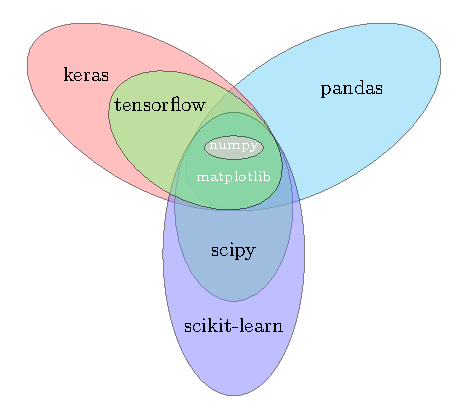
\includegraphics[width=\linewidth]{./src/figures/toolkits_set.pdf}
		}
		\caption[10mm]{Click Figure to view popular APIs for data mining.}
	\end{figure}
\end{minipage}%
\hfill%
\begin{minipage}{0.5\textwidth}
	\begin{itemize}
		\item[numpy] linear algebra algorithm library, operations on the n-dimensional array.
		\item[matplotlib] data visualization.
		\item[pandas] data structures and operations for manipulating tables.
		\item[scipy] optimization, interpolation, statistic, sparse matrix.
		\item[scikit-learn] Preprocessing, Clustering, Classification, Regression
		\item[tensorflow] Parallel Computing.
		\item[keras] Deep Learning. 
	\end{itemize}
\end{minipage}
\end{frame}


%=========================================================
\section{Example 1}

\subsection{Kaggle Dataset}
\begin{frame}
	\frametitle{Titanic - Machine Learning from Disaster}
	% The data has been split into two groups:
	% * training set (train.csv)
	% * test set (test.csv)
	% The training set should be used to build your machine learning models. For the training set, we provide the outcome (also known as the “ground truth”) for each passenger. Your model will be based on “features” like passengers’ gender and class. You can also use feature engineering to create new features.

	% The test set should be used to see how well your model performs on unseen data. For the test set, we do not provide the ground truth for each passenger. It is your job to predict these outcomes. For each passenger in the test set, use the model you trained to predict whether or not they survived the sinking of the Titanic.

	% We also include gender_submission.csv, a set of predictions that assume all and only female passengers survive, as an example of what a submission file should look like.
	\begin{flushleft}
		This is a classical data set in Kaggle, it consists of
		\begin{center}
			\begin{minipage}{0.8\textwidth}
				\begin{itemize}
					\item[train.csv] This table contains all the training data(features and labels).
					\item[test.csv] This table contains the feature attributes of the testing data.
					\item[{\tiny gender\_submission.csv}] This table contains the label attributes of the testing data.
				\end{itemize}
			\end{minipage}
		\end{center}
		While using python data mining toolkits, we do not have to know the exact meaning of each attribute or the background of the dataset, because the preprocessing and data visualization can help us parse the attributes.
	\end{flushleft}
\end{frame}

%---------------------------------------------------------
\subsection{Preprocessing: Read dataset and parse attributes}
\begin{frame}
	\frametitle{Read dataset and parse attributes}
	\begin{flushleft}
		When we already obtain the dataset, the first step is reading the dataset to the RAM.
	\end{flushleft}
	\begin{center}
		\textbf{\color{blue}\footnotesize train = pd.read\_csv("datasets/train.csv")}
	\end{center}
	\begin{flushleft}
		Combining data from two or more tables, based on the primary key.
	\end{flushleft}
	\begin{center}
		\textbf{\color{blue} \footnotesize
			test = pd.merge(~~~~~~~~~~~~~~~~~~~~~~~~~~~~~~~~~~~~~~~~~~~~~~~~~~~ \\
			left=pd.read\_csv("datasets/gender\_submission.csv"), \\
			right=pd.read\_csv("datasets/test.csv"),~~~~~~~~~~~~~~~~~ \\
			on="PassengerId")~~~~~~~~~~~~~~~~~~~~~~~~~~~~~~~~~~~~~~~~~ 
		}
	\end{center}
	\begin{block}{Remark}
	Pandas is a hybrid of Python and SQL language. Many python-based web frameworks(ex. Django) use Pandas instead of traditional SQL operations.
	\end{block}
	\begin{flushleft}
		It is convenient to parse all the fields by using this method
	\end{flushleft}
	\begin{center}
		\textbf{\color{blue}\footnotesize train.info()}
	\end{center}
\end{frame}

\begin{frame}
	\frametitle{Read dataset and parse attributes}
	\begin{flushleft}
		The main usage of printing this table is to help us to work with the missing data.
	\end{flushleft}
	\begin{center}
		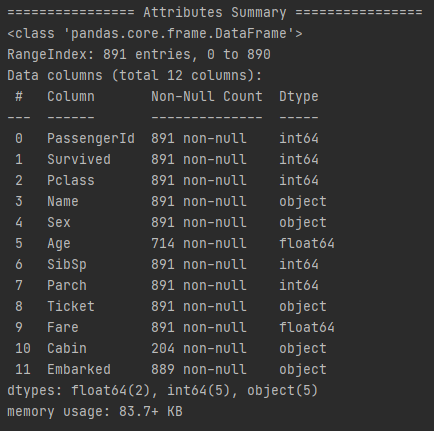
\includegraphics[width=0.55\linewidth]{./src/figures/1.png}
	\end{center}
\end{frame}

%---------------------------------------------------------
\subsection{Preprocessing: Working with Missing Data}
\begin{frame}
	\frametitle{Working with Missing Data}
	\begin{flushleft}
		Filling missing values with a new class
	\end{flushleft}
	\begin{center}
		\textbf{\color{blue}train["Cabin"] = train["Cabin"].fillna("None")}
	\end{center}
	\begin{flushleft}
		Filling missing values with the mean value
	\end{flushleft}
	\begin{center}
		\textbf{\color{blue}train["Age"] = train["Age"].fillna(train["Age"].mean())}
	\end{center}
	\begin{flushleft}
		Droping samples with missing values.
	\end{flushleft}
	\begin{center}
		\textbf{\color{blue}train = train.dropna()}
	\end{center}
	\begin{flushleft}
		Of course, we must do the same implementation in the testing dataset. \\
		After working with the missing data, It is convenient to view the statistics by one-line command.
	\end{flushleft}
	\begin{center}
		\textbf{\color{blue}print(train.describe()) \\ print(test.describe())}
	\end{center}
\end{frame}

\begin{frame}
	\frametitle{Working with Missing Data}
	\begin{flushleft}
		The main usage of printing this table is to help us to remove the noise.
	\end{flushleft}
	\begin{center}
		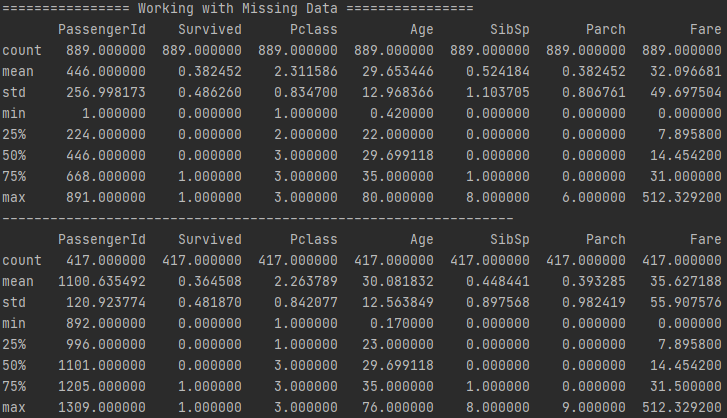
\includegraphics[width=0.9\linewidth]{./src/figures/2.png}
	\end{center}
\end{frame}

%---------------------------------------------------------
\subsection{Preprocessing: Noise Reduction}
\begin{frame}
	\frametitle{Noise Reduction}
	\begin{flushleft}
		From the statistics above, we find that
		\begin{itemize}
			\item train["Parch"].mean() $\approx$ test["Parch"].mean()
            \item train["Parch"].std() $\approx$ test["Parch"].std()
            \item train["Parch"].max() $\sim \approx$ train["Parch"].max()
		\end{itemize}
		It implices that there exists noise in the attribute `Parch`. One-line command to remove such noise.(It is equivalent to the `where` command in SQL language)
	\end{flushleft}
	\begin{center}
		\textbf{\color{blue}test = test[test["Parch"] $\le$ 8]}
	\end{center}
	\begin{flushleft}
		We also notice that $train["Fare"].std() \gg 1$, it implices that there exists noise in the attribute `Fare`. We can use cluster algorithm to remove such noise.
	\end{flushleft}
\end{frame}

%---------------------------------------------------------
\subsection{Data Visualization}
\begin{frame}
	\frametitle{Data Visualization}
	\begin{flushleft}
		Except printing the `describe` table, we can also use data visualization to help us with data preprocessing.
	\end{flushleft}
	\begin{center}
		\begin{figure}
	    \foreach[count=\i] \row/\col in {
	      0/0, 0/1, 0/2,
	      1/0, 1/1, 1/2,
	      2/0, 2/1, 2/2
	    } {%
	      \begin{subfigure}[p]{0.24\textwidth}
	          \includegraphics[width=\linewidth]{./src/figures/4_\i.png}
	          % \caption{ }
	      \end{subfigure}
	      \ifthenelse{\col=2}{\\}{\hfill}
			}
		\end{figure}
	\end{center}
\end{frame}

%---------------------------------------------------------
\subsection{Preprocessing: Data Reduction}
\begin{frame}
	\frametitle{Data Reduction}
	\begin{flushleft}
		From the data visualization above, we find that the attribute `Cabin` contains too many classes, make the correlation analysis to check the validity of this attribute. \\
		\textbf{\color{blue}
			cross\_table = pd.crosstab(train["Cabin"].values, train["Survived"].values) \\
			if stats.chi2\_contingency(observed=cross\_table.values)[1] $<$ 0.05:\\
	    \quad train = train.drop(columns=["Cabin"]) \\
	    \quad test = test.drop(columns=["Cabin"])
		} \\
		Since $p_{val} = 2.71e-06$, we need drop this field. Check the information of the two datasets again to have a view of the attributes.
	\end{flushleft}
	\begin{center}
		\textbf{\color{blue}\footnotesize train.info()}\\
		\textbf{\color{blue}\footnotesize test.info()}~~
	\end{center}
\end{frame}

\begin{frame}
\frametitle{Data Reduction}
	\begin{flushleft}
		These tables show us, the attributes contain continuous values and discrete values, so we have to convert them into the same datatype in the next step. 
	\end{flushleft}
	\begin{center}
		\begin{figure}
			\begin{subfigure}[p]{0.48\textwidth}
	        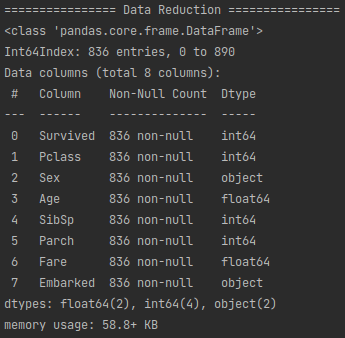
\includegraphics[width=\linewidth]{./src/figures/5_1.png}
	        \caption{Train}
	    \end{subfigure} \hfill
			\begin{subfigure}[p]{0.48\textwidth}
	        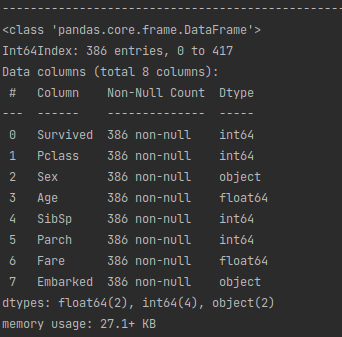
\includegraphics[width=\linewidth]{./src/figures/5_2.png}
	        \caption{Test}
	    \end{subfigure}
	  \end{figure}
	\end{center}
\end{frame}

%---------------------------------------------------------
\subsection{Preprocessing: Partition Continuous Features into Discrete Values}
\begin{frame}
	\frametitle{Partition Continuous Features into Discrete Values}
	\begin{flushleft}
		By using the histogram above, the continuous variables can be binning easily.
	\end{flushleft}
	\begin{center}
		\textbf{\color{blue} \footnotesize
			train["Age"] = (train["Age"] // 16) * 16~~ \\
			train["Fare"] = (train["Fare"] // 19) * 19 \\
			test["Age"] = (test["Age"] // 16) * 16~~~~ \\
			test["Fare"] = (test["Fare"] // 19) * 19~~
		}
	\end{center}
	\begin{block}{Remark}
		\begin{itemize}
	  	\item For different attributes, we can use different standards in binning the values. But for the same attribute in different datasets, we must obey the same rule when binning the values. 
	  	\item When we using clustering methods to discrete the continuous values, we should make sure the class is sorted in order.
		\end{itemize}
	\end{block}
	\begin{flushleft}
		Now the data preprocessing is completed. Let's view these two tables
	\end{flushleft}
	\begin{center}
		\textbf{\color{blue} \footnotesize
			print(train) \\
			print(test)~
		}
	\end{center}
\end{frame}

\begin{frame}
\frametitle{Data Reduction}
\begin{center}
	\begin{figure}
    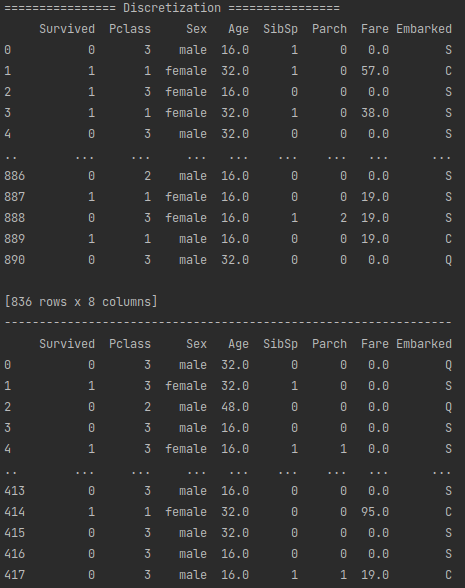
\includegraphics[width=0.5\linewidth]{./src/figures/6.png}
  \end{figure}
\end{center}
\end{frame}

%---------------------------------------------------------
\subsection{Classification: Decision Tree}
\begin{frame}
	\frametitle{Decision Tree}
	\begin{flushleft}
		\textbf{Step 1:} Converting tables to n-dimensional arrays \\
		\textbf{\color{blue} \scriptsize
			train['Sex'] = train['Sex'].map({'male': 0, 'female': 1}).astype(int) \\
			train['Embarked'] = train['Embarked'].map({'S': 0, 'C': 1, 'Q': 2}).astype(int) \\
			x\_train = train[["Pclass", "Sex", "Age", "SibSp", "Parch", "Fare", "Embarked"]].values \\
			y\_train = train["Survived"].values \\
		}
		Of course, we must do the same implementation in the testing dataset. \\
		\textbf{Step 2:} Training the model \\
		\textbf{\color{blue} \scriptsize
			decision\_tree = tree.DecisionTreeClassifier() \\
			decision\_tree.fit(x\_train, y\_train) \\
		}
		\textbf{Step 3:} Computing the accuracy \\
		\textbf{\color{blue} \scriptsize
			y\_pred = decision\_tree.predict(x\_test) \\
			print("Train accuracy: $\{\}$ \%".format(round(decision\_tree.score(x\_train, y\_train) * 100, 2))) \\
			print("Test accuracy: $\{\}$ \%".format(round(decision\_tree.score(x\_test, y\_test) * 100, 2)))
		}
	\end{flushleft}
	\begin{center}
		\begin{figure}
	    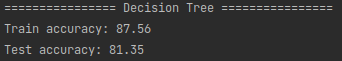
\includegraphics[width=0.5\linewidth]{./src/figures/7.png}
	  \end{figure}
	\end{center}
\end{frame}

\begin{frame}
	\frametitle{Decision Tree}
	\begin{flushleft}
		\textbf{Step 4:} Printing the Decision Tree \\
		\textbf{\color{blue} \scriptsize
			print(tree.export\_text(decision\_tree, feature\_names=["Pclass", "Sex", "Age", "SibSp", "Parch", "Fare", "Embarked"]))
		}
	\end{flushleft}
	\begin{center}
		\begin{figure}
	    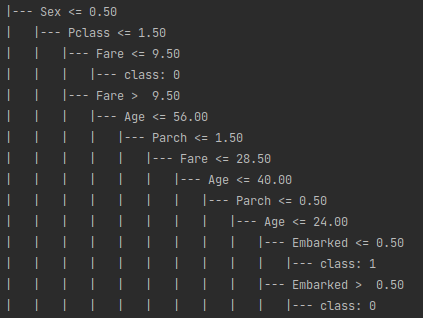
\includegraphics[width=0.5\linewidth]{./src/figures/7_1.png}
	  \end{figure}
	\end{center}
\end{frame}


%=========================================================
\section{Example 2}

%---------------------------------------------------------
\subsection{Preprocessing: Encoding Categorical Attributes}
\begin{frame}
	\frametitle{Encoding Categorical Attributes}
	% The second example is doing the same classification task in the same dataset, but this time I will use the neural network to do this work.
	\begin{flushleft}
		Before using any Neural Network to do the classification task, we have to convert the Categorical Values to vectors. The most popular encoding algorithm is one-hot. It is widely used in classification tasks.
	\end{flushleft}
	\begin{center}
		\textbf{\color{blue}
			encoder = preprocessing.OneHotEncoder()~~~~~~~~~~~~~~~~~~ \\
			encoder.fit(train[["Pclass", "Sex", "Embarked"]].values)
		}
	\end{center}
	\begin{block}{Example}
		The output of encoder.transform([[3, "male", "Q"], [3, "female", "S"]] is 
		\begin{center}
			\begin{figure}
		    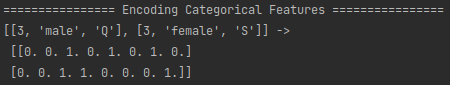
\includegraphics[width=0.5\linewidth]{./src/figures/8.png}
		  \end{figure}
		\end{center}
	\end{block}
\end{frame}

%---------------------------------------------------------
\subsection{Preprocessing: Dimensionality Reduction}
\begin{frame}
	\frametitle{Dimensionality Reduction}
	\begin{flushleft}
		The one-hot encoder will greatly increase the dimension of features, so we can use PCA to reduce it. PCA is an SVD-based method. Its core is to remain the parts with high Singular Values which is similar to the image compression technology.
	\end{flushleft}
	\begin{center}
			\begin{figure}
		    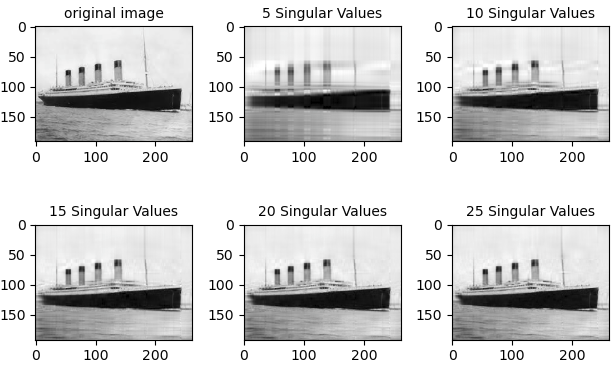
\includegraphics[width=0.5\linewidth]{./src/figures/11.png}
		  \end{figure}
		\end{center}
	\begin{block}{Remark}
		For Deep Learning, PCA is not necessary.
	\end{block}
\end{frame}

%---------------------------------------------------------
\subsection{Classification: MLP}
\begin{frame}
	\frametitle{MLP}
	\begin{flushleft}
		\textbf{Step 1:} Converting tables to n-dimensional arrays \\
		\textbf{\color{blue} \scriptsize
			x\_train = np.concatenate([ \\
		  ~~~~encoder.transform(train[["Pclass", "Sex", "Embarked"]].values).toarray(), \\
		  ~~~~train[["Age", "SibSp", "Parch", "Fare"]].values \\
			], axis=1) \\
			y\_train = train["Survived"].values \\
		}
		Of course, we must do the same implementation in the testing dataset. \\
		\textbf{Step 2:} Build the model \\
		\textbf{\color{blue} \scriptsize
			model = tf.keras.models.Sequential([               \\
		  ~~~~tf.keras.layers.Dense(512, activation='relu'), \\
		  ~~~~tf.keras.layers.BatchNormalization(),          \\
		  ~~~~tf.keras.layers.Dense(256, activation='relu'), \\
		  ~~~~tf.keras.layers.BatchNormalization(),          \\
		  ~~~~tf.keras.layers.Dense(128, activation='relu'), \\
		  ~~~~tf.keras.layers.BatchNormalization(),          \\
		  ~~~~tf.keras.layers.Dense(2)                       \\
			])                                                 \\
			model.compile(                                     \\
		  ~~~~optimizer=tf.keras.optimizers.Adam(0.005),     \\
		  ~~~~loss=tf.keras.losses.SparseCategoricalCrossentropy(from\_logits=True), \\
		  ~~~~metrics=['accuracy']) \\
		}
	\end{flushleft}
\end{frame}

\begin{frame}
	\frametitle{MLP}
	\begin{flushleft}
		\textbf{Step 3:} Training the model \\
		\textbf{\color{blue} \scriptsize
			model.fit( \\
			~~~~x\_train, y\_train, batch\_size=4, epochs=20, \\
			~~~~validation\_data=(x\_test,  y\_test), \\
			~~~~callbacks=[ \\
			~~~~~~~~tf.keras.callbacks.LearningRateScheduler(lambda epoch, lr: 0.75 ** (epoch // 10) * lr, verbose=1), \\
			~~~~~~~~tf.keras.callbacks.TensorBoard(log\_dir="logs/" + datetime.now().strftime("\%Y\%m\%d-\%H\%M\%S"), histogram\_freq=1) \\
			~~~~], \\
			) \\
		}
		The computer will print the training logs in the terminal
	\end{flushleft}
	\begin{center}
		\begin{figure}
	    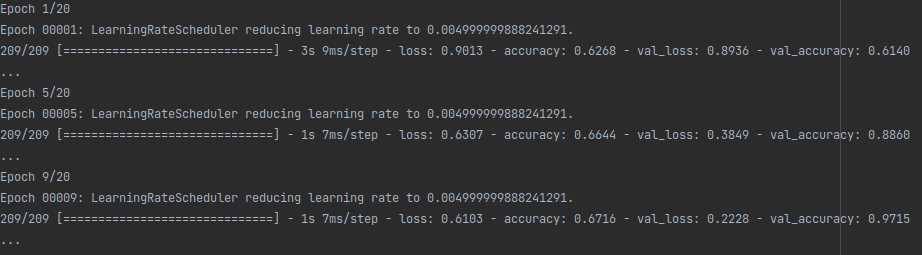
\includegraphics[width=0.8\linewidth]{./src/figures/9.png}
	  \end{figure}
	\end{center}
\end{frame}

\begin{frame}
	\frametitle{Tensorboard}
	\begin{flushleft}
		\textbf{Step 4:} Open the tensorboard to view the data plot of training logs in a web browser. \\
	\end{flushleft}
	\begin{center}
		\textbf{\$ \color{blue} tensorboard --logdir logs}
	\end{center}
	\begin{center}
		\begin{figure}
        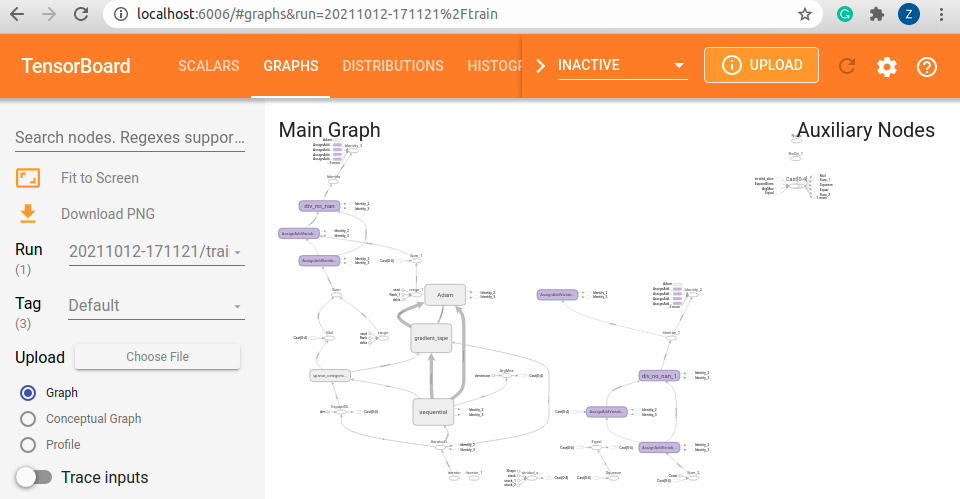
\includegraphics[width=0.85\linewidth]{./src/figures/10_2.png}
        \caption{Computational Graph}
		\end{figure}
	\end{center}
\end{frame}

\begin{frame}
	\frametitle{Tensorboard}
	\begin{center}
		\begin{figure}
        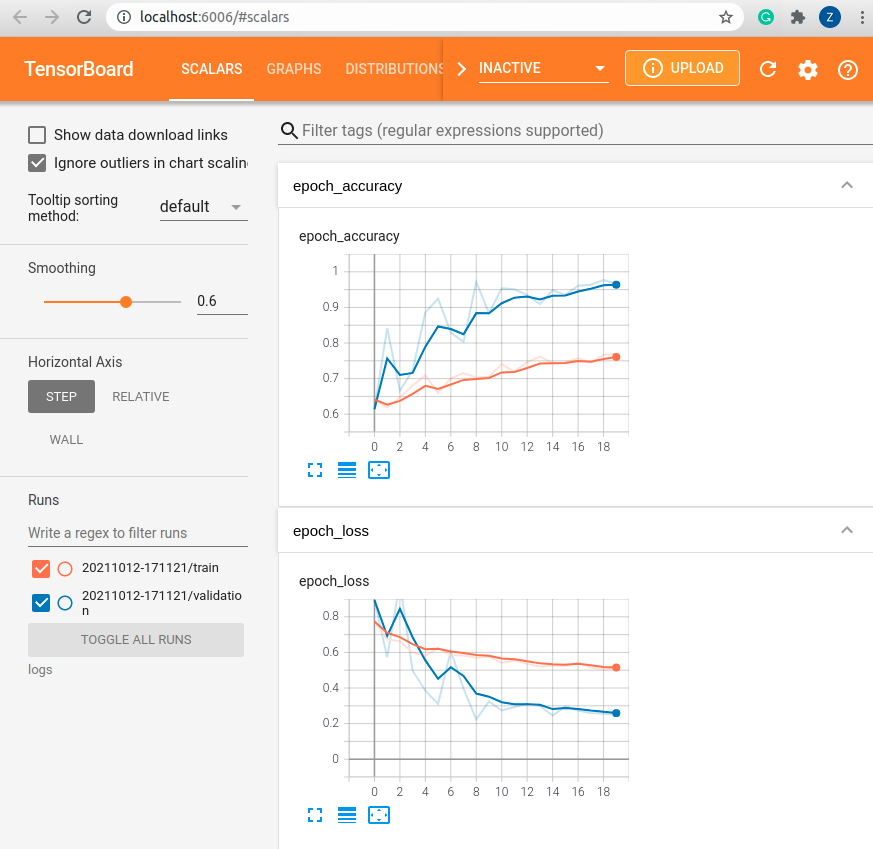
\includegraphics[width=0.6\linewidth]{./src/figures/10_1.png}
        \caption{Loss and Accuracy}
		\end{figure}
	\end{center}
\end{frame}

\begin{frame}
	\frametitle{Tensorboard}
	\begin{center}
		\begin{figure}
        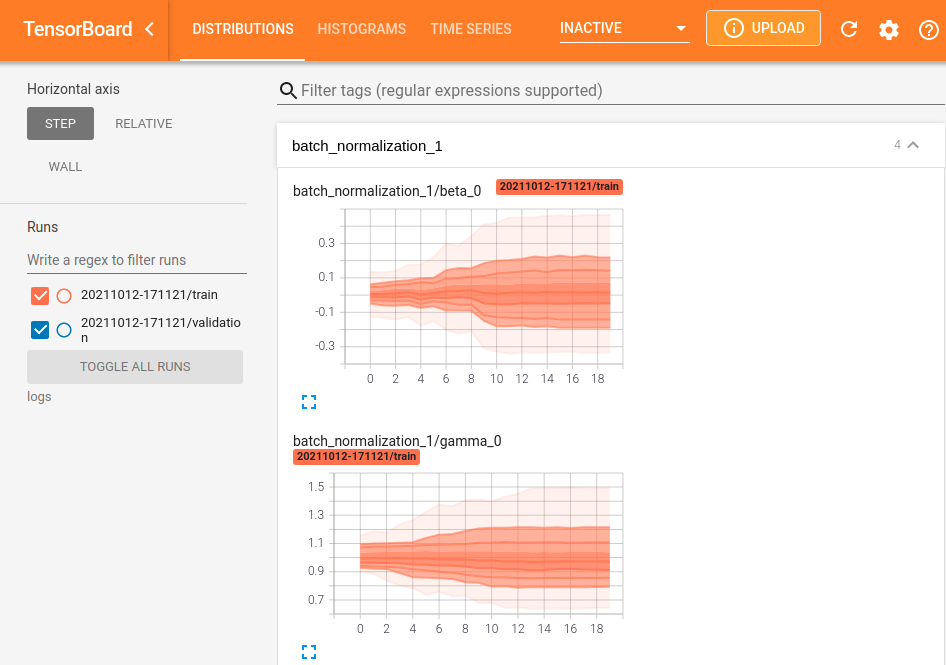
\includegraphics[width=0.8\linewidth]{./src/figures/10_3.png}
        \caption{Distibutions of model parameters}
		\end{figure}
	\end{center}
\end{frame}

\begin{frame}
	\frametitle{Tensorboard}
	\begin{center}
		\begin{figure}
        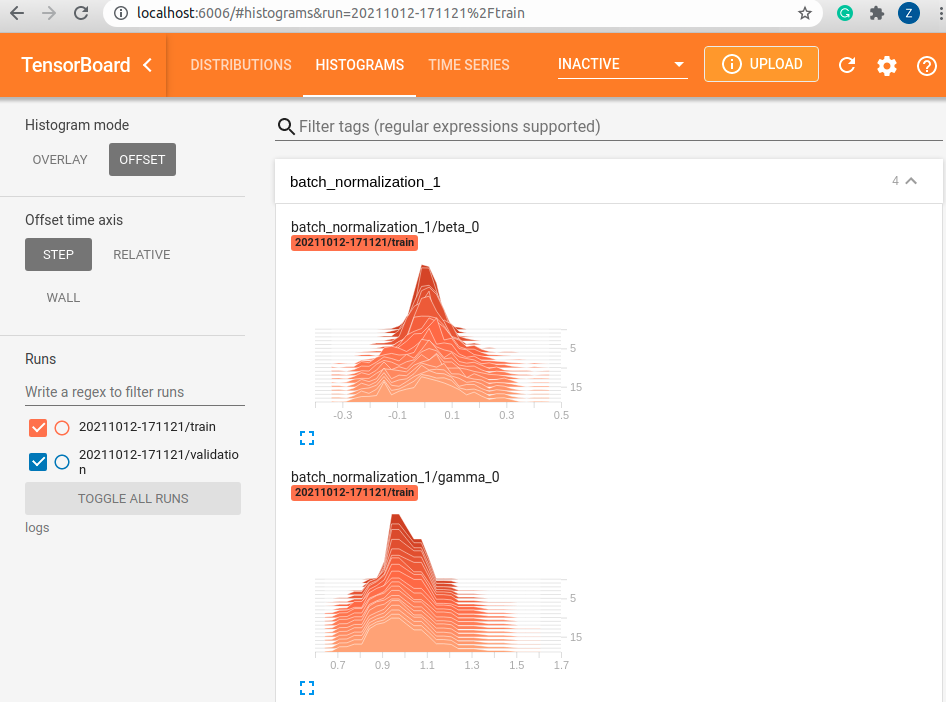
\includegraphics[width=0.8\linewidth]{./src/figures/10_4.png}
        \caption{Histogram of model parameters}
		\end{figure}
	\end{center}
\end{frame}


\end{document}